% !TEX root = _individual/trtBackground.tex

%%%%%%%%%%%%%%%%%%%%%%%%%%%%%%%%%%%%%%%%%%%%%%%%%%%%%%%%%%%%%%%%%%%%%%%%%%%%%%%%
\chapter{Background: Thermal Radiative Transfer}

Thermal radiative transfer (TRT) is the nonlinear process describing the
dominant form of energy transfer in a very hot material, such as the interior
of a star or the
target of a laser fusion experiment. The equations describing TRT are
time-dependent, contain strong nonlinearities, and reside in a large phase
space. These difficulties make TRT the subject of significant work in methods
development.

A full representation of the physics in
those high-energy-density regimes often includes the consideration of moving
relativistic materials, different electron and ion temperatures, photon
scattering, and thermal conduction in the material \cite{Mih1984}. However,
much theoretical work in the field neglects these complex phenomena by
\prelistpar
\begin{itemize}
  \item working in a fixed medium, disregarding material advection;
  \item assuming local thermodynamic equilibrium (LTE), which uses a single
    material temperature;
  \item neglecting photon scattering, which VERIFY THIS tends to be small for
    very hot materials; and
  \item neglecting thermal conduction, since energy transfer is dominated by
    radiative transfer in the temperature regimes we consider.
\end{itemize}

A further simplification often used for methods development is the ``gray''
approximation to the frequency dependence. Analogous to the one-group
approximation for neutron transport, the full transport equation is integrated
over all frequencies, and the opacities are averaged with some \emph{a priori}
weighting function. The commonly used Rosseland mean satisfies a radiation
diffusion equation found in an asymptotic analysis of the thermal radiative
transfer equations \cite{Lar1983a} and is therefore the best choice for a
method that resembles diffusion.

%%%%%%%%%%%%%%%%%%%%%%%%%%%%%%%%%%%%%%%%%%%%%%%%%%%%%%%%%%%%%%%%%%%%%%%%%%%%%%%%
\section{TRT equations}
After the simplifications, the thermal radiative transfer process can be
described by
\begin{subequations} \label{eqs:fullGrayTRT}
the radiative transfer equation,
\begin{equation} \label{eq:fullGrayTransport}
  \frac{1}{c} \pder{I}{t}
  + \vec{\Omega} \vd \del I +
 \sigma I
  = \frac{\sigma c U_r}{4\pi} 
  + \frac{c Q}{4\pi} \,,
\end{equation}
and the material energy balance equation
\begin{equation} \label{eq:fullGrayMaterial}
  \pder{U_m}{t} = \sigma \int_{4\pi}  I \ud \Omega - \sigma c U_r
  %= \sigma \phi - \sigma c U_r
  \,.
\end{equation}
\end{subequations}

The notation and omitted parameters in Eqs.~\eqref{eqs:fullGrayTRT} are:
\begin{alignat*}{2}
  I &= I(\vec{x}, \vec{\Omega}, t) &&= \text{the angle-dependent
  radiation intensity,}
%  \\
%  \phi &= \phi(\vec{x}, t) &&= \text{the zeroth angular moment of the radiation
%  intensity,}
  \\
  T &= T(\vec{x}, t) &&= \text{the temperature of the material,}
  \\
  \sigma &= \sigma(\vec{x}, T) &&= \text{the absorption opacity,} 
  \\
  Q &= Q(\vec{x}) &&= \text{an extraneous isotropic radiation energy source,}
  \\
  U_m &= U_m(\vec{x}, T) &&= \text{the material energy density,}
  \\
  U_r &= U_r(\vec{x}, T) &&= \text{the equilibrium radiation energy density of
  the material,}
  \\
  c_v &= c_v(\vec{x}, T) &&= \text{the specific heat capacity of a material,}
  \\
  c& &&= \text{the speed of light.}
\end{alignat*}
The ``equilibrium radiation energy density'' of a material is a scaled integral
of the Planckian emission function:
\begin{subequations} \label{eqs:materialU}
\begin{equation} \label{eq:radEnergyDens}
  U_r(T) \equiv aT^4 = \frac{1}{c} \int_{4\pi} \int_{0}^{\infty}B(\nu, T) \ud
  \nu \ud \Omega \,.
\end{equation}
The material energy density is related only to the material's temperature:
\begin{equation} \label{eq:matEnergyDens}
  U_m(T) = \int_{0}^{T} c_v(T') \ud T' \,.
\end{equation}
The specific heat capacity $c_v(T)$ is the amount of energy per unit
volume needed to change the material's temperature.
\end{subequations}
%The zeroth moment of $I$ is equal to the radiation energy density scaled by the
%speed of light:
%\begin{equation*}
%  \phi(\vec{x}, t) = \int_{4\pi} I(\vec{x}, \vec{\Omega}, t) \ud \Omega
%  = \int_{4\pi} c [h \nu] N(\vec{x}, \vec{\Omega}, t) \ud \Omega
%  = c \RadEn(\vec{x}, t)\,.
%\end{equation*}
%Here, $N$ is the photon density, $h\nu$ is the energy of a single photon, and
%$E$ is the radiation energy density.

%%%%%%%%%%%%%%%%%%%%%%%%%%%%%%%%%%%%%%%%%%%%%%%%%%%%%%%%%%%%%%%%%%%%%%%%%%%%%%%%
\section{Radiation transport approximations}\label{sec:trtApproxMethods}

The large phase space and nonlinearity of Eqs.~\eqref{eqs:fullGrayTRT} makes a
direct solution intractable except for the simplest of problems
\cite{Su1997,Mos2006}. A more complete overview of the approximations is given
in \cite{Bru2002,Ols2000,Wol2008}.

All of the approximations trade speed for accuracy. The fewer unknowns a method
has, the easier it is to solve.

%%%%%%%%%%%%%%%%%%%%%%%%%%%%%%%%%%%%%%%%
\subsection{Implicit Monte Carlo}

%%%%%%%%%%%%%%%%%%%%%%%%%%%%%%%%%%%%%%%%
\subsection{Discrete ordinates}

%%%%%%%%%%%%%%%%%%%%%%%%%%%%%%%%%%%%%%%%
\subsection{Spherical harmonics}

%%%%%%%%%%%%%%%%%%%%%%%%%%%%%%%%%%%%%%%%
\subsection{Diffusion}\label{sec:diffusion}

%%%%%%%%%%%%%%%%%%%%%%%%%%%%%%%%%%%%%%%%
\subsection{Flux-limited diffusion}

\subsubsection{Flux limiters}

\subsubsection{Flux limiter discretization}
\cite{Ols2007}

%%%%%%%%%%%%%%%%%%%%%%%%%%%%%%%%%%%%%%%%%%%%%%%%%%%%%%%%%%%%%%%%%%%%%%%%%%%%%%%%
\section{Semi-implicit linearization}

To solve the TRT equations with deterministic methods,\footnote{The Implicit
Monte Carlo scheme of Fleck and Cummings \cite{Fle1971} gives a result very
similar to the semi-implicit discretization. The difference is that Monte
Carlo does not need to approximate the time dependence implicitly.} we use the
semi-implicit time
discretization scheme \cite{Kno1999a,Kno2001,Low2004} where some important
unknowns are treated implicitly in
time, and other unknowns are treated explicitly. By choosing the intensity $I$
and equilibrium radiation energy density $U_r$ to be the implicit variables and 
by treating the opacity $\sigma$ and another material property explicitly,
Eqs.~\eqref{eqs:fullGrayTRT} can be formulated as a time-dependent linear
transport equation over a time step $t^n < t < t^{n+1}$.

\subsection{Linearizing the material energy equation}
First, we define a parameter $\beta$ as a function of Eqs.~\eqref{eqs:materialU}:
\begin{equation} \label{eq:beta}
  \beta(T) = \pder{U_r}{U_m} 
  = \pder{U_r}{T} \Bigg/ \pder{U_m}{T}
  = \frac{4 a T^3}{c_v(T)} \,.
\end{equation}
The chain rule allows the left hand side of Eq.~\eqref{eq:fullGrayMaterial} to be
expressed without approximation in terms of the equilibrium radiation energy
density $U_r$:
\begin{equation*}
  \pder{U_m}{t} = \pder{U_m}{U_r} \pder{U_r}{t} = \frac{1}{\beta(T)}
  \pder{U_r}{t} = \sigma \int_{4\pi}  I \ud \Omega - \sigma c U_r \,.
\end{equation*}
The first approximation is to ``freeze'' the parameter $\beta$ at the beginning-of-time-step temperature $T^n$:
\begin{equation}\label{eq:frozenBeta}
  \frac{1}{\beta^n}
  \pder{U_r}{t} \approx \sigma \int_{4\pi}  I \ud \Omega - \sigma c U_r \,.
\end{equation}
Because the approximation to $\beta$ is an approximation to the rate of change
in material energy, this equation no longer conserves the system's total
energy. To enforce conservation of energy over a time step, we must set the
material energy change over a time step to the time-integrated approximation:
\begin{align}
  \nonumber
  \int_{t^n}^{t^{n+1}}  \pder{U_m}{t}\ud t &= \frac{1}{\beta^n}
  \int_{t^n}^{t^{n+1}} \pder{U_r}{t}\ud t
  \\
  \nonumber
  U_m^{n+1} - U_m^n &= \frac{1}{\beta^n} \left[ U_r^{n+1} - U_r^n \right]
  \\
  \label{eq:matenConservationUpdate}
  U_m^{n+1} &=  U_m^n + \frac{U_r^{n+1} - U_r^n}{\beta^n}\,.
\end{align}
%Thus, the expression of $\tpder{U_m}{t}$ in terms of $\tpder{U_r}{t}$

The next approximation is to explicitly freeze the opacity $\sigma$ in
Eq.~\eqref{eq:frozenBeta}:
\begin{equation*}
  \frac{1}{\beta^n}
  \pder{U_r}{t} \approx \sigma^n \int_{4\pi}  I \ud \Omega - \sigma^n c U_r \,.
\end{equation*}
Now we can time-average the material equation to express it in terms of two
simple time-average unknowns. Operating by
$\frac{1}{\Delta_t^n}\int_{t_n}^{t^{n+1}} (\cdot) \ud t$,
\begin{equation*}
  \frac{1}{\beta^n}
  \frac{U_r^{n+1} - U_r^n}{\Delta_t^n} = \sigma^n \int_{4\pi} \left[
  \frac{1}{\Delta_t^n}\int_{t_n}^{t^{n+1}} I\ud t
  \right] \ud \Omega - \sigma^n c \left[
  \frac{1}{\Delta_t^n}\int_{t_n}^{t^{n+1}} U_r \ud t \right]\,.
\end{equation*}
Next, we apply the implicit Euler approximation to $U_r(\vec{x}, \vec{\Omega},
t)$ and $I(\vec{x}, \vec{\Omega}, t)$ by setting their time-averaged values to
the values at $t^{n+1}$:
\begin{equation} \label{eq:semiImplicitMaterial}
  \frac{1}{\beta^n(\vec{x})}
  \frac{U_r^{n+1}(\vec{x}) - U_r^n(\vec{x})}{\Delta_t^n}
  = \sigma^n(\vec{x}) \int_{4\pi} I^{n+1}(\vec{x}, \vec{\Omega})\ud \Omega
  - c \sigma^n(\vec{x}) U_r^{n+1}(\vec{x}) \,.
\end{equation}

We solve Eq.~\eqref{eq:semiImplicitMaterial} for $U_r^{n+1}$ in order to
eliminate the implicit dependence of the transport equation on the material
energy equation.
\begin{align} \nonumber
  U_r^{n+1} - U_r^n
  &= \beta^n \Delta_t^n \sigma^n\int_{4\pi} I^{n+1}\ud \Omega
   - c \beta^n \Delta_t^n \sigma^n U_r^{n+1}
   \\ \nonumber
  U_r^{n+1} [ 1 + c \beta^n \Delta_t^n \sigma^n ]
  &= \beta^n \Delta_t^n \sigma^n\int_{4\pi} I^{n+1}\ud \Omega + U_r^n
   \\ \nonumber
  U_r^{n+1}
  &= \frac1c \frac{ c \beta^n \Delta_t^n \sigma^n }{ 1 + c \beta^n \Delta_t^n \sigma^n}
  \int_{4\pi} I^{n+1}\ud \Omega + \frac1{ 1 + c \beta^n \Delta_t^n \sigma^n}
  U_r^n
  \\ \nonumber
  U_r^{n+1}
  &= \left[1 - \frac{1 }{ 1 + c \beta^n \Delta_t^n \sigma^n} \right]
  \int_{4\pi} I^{n+1}\ud \Omega + \frac1{ 1 + c \beta^n \Delta_t^n \sigma^n}
  U_r^n
  \\ \label{eq:urNPlusOne}
  U_r^{n+1}
  &= \left(1 - f^n\right) \frac1c \int_{4\pi} I^{n+1}\ud \Omega + f^n U_r^n
\end{align}
where
\begin{equation} \label{eq:fleckFactor}
  f^n = f^n(\vec{x}) \equiv \left[ 1 + \beta^n c \Delta_t^n \sigma^n
  \right]\inv \,.
\end{equation}
This semi-implicit formulation is very similar to the linearization in Fleck
and Cummings' IMC method \cite{Fle1971}, although they leave the intensity $I$
in a time-dependent form.

\subsection{Linearizing the transport equation}
The next step is apply similar approximations to the nonlinear radiation
transport equation~\eqref{eq:fullGrayTransport}. As with the material equation,
the
opacities are ``frozen'' at their beginning-of-time-step values $\sigma^n$, and
the equation is time-averaged:
\begin{multline*}
  \frac{1}{c} \frac{I^{n+1} - I^n}{\Delta_t^n}
  + \vec{\Omega} \vd \del \left[
  \frac{1}{\Delta_t^n}\int_{t_n}^{t^{n+1}} I\ud t
  \right] +
 \sigma^n \left[
  \frac{1}{\Delta_t^n}\int_{t_n}^{t^{n+1}} I\ud t
  \right]
  \\
  = \frac{\sigma^n c}{4\pi} \left[
  \frac{1}{\Delta_t^n}\int_{t_n}^{t^{n+1}} U_r \ud t \right]
  + \frac{1}{4\pi}\left[
  \frac{1}{\Delta_t^n}\int_{t_n}^{t^{n+1}} Q \ud t \right] \,.
\end{multline*}
Since the extraneous energy source $Q$ is assumed to be known \emph{a priori},
we let its time-averaged value be $Q^n$. As in the material equation, we apply
the implicit Euler approximation to $I$ and $U_r$:
\begin{equation*}
  \frac{1}{c} \frac{I^{n+1} - I^n}{\Delta_t^n}
  + \vec{\Omega} \vd \del I^{n+1}
 + \sigma^n I^{n+1}
 = \frac{\sigma^n c}{4\pi} U_r^{n+1}
  + \frac{c}{4\pi} Q^n \,.
\end{equation*}
Finally, we substitute $U_r^{n+1}$ from Eq.~\eqref{eq:urNPlusOne},
which was derived from the material equation Eq.~\eqref{eq:fullGrayMaterial}:
\begin{align}\nonumber
  \frac{1}{c} \frac{I^{n+1} - I^n}{\Delta_t^n}
  + \vec{\Omega} \vd \del I^{n+1}
 + \sigma^n I^{n+1}
 &= \frac{\sigma^n c}{4\pi} \left[ \left(1 - f^n\right) \frac1c \int_{4\pi} I^{n+1}\ud \Omega + f^n U_r^n \right]
  + \frac{c}{4\pi} Q^n
  \\ \label{eq:linearizedGrayTransport}
  \frac{1}{c} \frac{I^{n+1} - I^n}{\Delta_t^n}
  + \vec{\Omega} \vd \del I^{n+1}
 + \sigma^n I^{n+1}
 &=  \left(1 - f^n\right) \sigma^n \frac{1}{4\pi} \int_{4\pi} I^{n+1}\ud \Omega
 + \frac{1}{4\pi} f^n \sigma^n c U_r^n
  + \frac{1}{4\pi} c Q^n \,.
\end{align}

\subsection{Comments}\label{sec:trtLinearizedComments}
If we compare Eq.~\eqref{eq:linearizedGrayTransport} to a temporally implicit
discretization of a monoenergetic linear transport problem with isotropic
scattering,
\begin{equation*}
  \frac{1}{v} \frac{\psi^{n+1} - \psi^n}{\Delta_t^n} 
  + \vec{\Omega} \vd \del \psi^{n+1}
 + \Sigma_t \psi^{n+1}
 = \frac{1}{4\pi} \int_{4\pi} \psi^{n+1}\ud \Omega
  + \frac{1}{4\pi} q \,,
\end{equation*}
we find equivalences between the two:
\begin{alignat*}{2}
  I &\leftrightarrow \psi &&= \text{the angular flux,}
  \\
  \sigma^n &\leftrightarrow \Sigma_t &&= \text{the total cross section,}
  \\
  \left(1 - f^n\right) \sigma^n &\leftrightarrow \Sigma_s &&= \text{the scattering cross
  section,} 
  \\
  f^n \sigma^n c U_r^n + c Q^n &\leftrightarrow q &&= \text{the isotropic source for time
  step $n$,}
  \\
  v   &\leftrightarrow c &&= \text{the particle velocity.}
\end{alignat*}
Even though the original radiation transport equation was purely
absorbing, the linearization scheme created a ``pseudoscattering''
term that essentially emulates the absorption and reemission of
radiation during a time step. The literature sometimes refers to an
``effective scattering opacity,''
$\sigma_\text{es}^n \equiv \left(1 - f^n\right) \sigma^n$.

Furthermore, if we take the zeroth angular moment of
Eq.~\eqref{eq:linearizedGrayTransport} and let $\phi^{n+1}(\vec{x}) \equiv
\frac{1}{4\pi} \int_{4\pi} I^{n+1}\ud \Omega$, then
\begin{align*}
  \frac{1}{c} \frac{\phi^{n+1} - \phi^n}{\Delta_t^n}
  + \del \vd \vec{F}^{n+1}
 + \sigma^n \phi^{n+1}
 &=  \left(1 - f^n\right) \sigma^n \phi^{n+1} +f^n \sigma^n c U_r^n
  + c Q^n
  \\
  \frac{1}{c} \frac{\phi^{n+1} - \phi^n}{\Delta_t^n}
  + \del \vd \vec{F}^{n+1} + f^n\sigma^n \phi^{n+1}
 &=  f^n \sigma^n c U_r^n + c Q^n\,.
\end{align*}
Thus, $f^n\sigma^n$ is sometimes known as the ``effective absorption opacity''
$\sigma_\text{ea}^n$.

\subsection{Solution process summary}
The time-dependent radiation solution is stored in the linear time-dependent
transport solver. The material energy $U_m$ must be stored, but the
material temperature can be either stored (highly recommended because of its
frequent use) or calculated on the fly from $U_m$ by inverting the integral in
Eq.~\eqref{eq:matEnergyDens}.

For the $n$th time step, given the initial radiation field $I^{n}$ and the
initial material energy density $U_m^n$, the solution process follows.
\prelistpar
\begin{enumerate}
  \item Linearize the system. Using the starting temperature $T^n$, calculate
    the frozen $\sigma^n$ and $\beta^n$ in each spatial cell. Use
    Eq.~\eqref{eq:fleckFactor} to calculate $f^n$, which in turn is used to
    calculate the linearized isotropic source $f^n \sigma^n c U_r^n + c Q^n$
    and the effective scattering cross section $\left(1 - f^n\right) \sigma^n$.
    If using a diffusion method to approximate the transport solution, the
    absorption cross sections and diffusion coefficients must be recalculated.
  \item Solve the linear transport problem for $\psi^{n+1}=I^{n+1}$. The new
    radiation
    temperature can optionally be calculated:
    \begin{equation*}
      a (T_\text{rad}^{n+1})^4 = \frac{1}{c} \int_{4\pi} I^{n+1}
      \ud \Omega
%      \lra
%      (T_\text{rad}^{n+1})^4 = \frac{1}{ac} \phi^{n+1}
      \lra
      T_\text{rad}^{n+1}(\vec{x}) = \left[ \frac{\phi^{n+1}(\vec{x})}{ac} \right]^{1/4}\,.
    \end{equation*}
  \item Update the material temperature. From Eq.~\eqref{eq:urNPlusOne}
    we can calculate the linearized estimate of $U_r^{n+1}$:
    \begin{equation*}
      U_r^{n+1} = \left(1 - f^n\right) \frac1c \phi^{n+1}  + f^n U_r^n\,.
    \end{equation*}
    However, because of the linearization of $\beta$, $U_r^{n+1} \ne a
    (T^{n+1})^4$. Instead, to calculate the material temperature, we must use
    Eq.~\eqref{eq:matenConservationUpdate}. Substituting
    Eq.~\eqref{eq:urNPlusOne} into Eq.~\eqref{eq:matenConservationUpdate}
    and simplifying gives
    \begin{equation}\label{eq:matenConservationUpdate2}
      U_m^{n+1} =  U_m^n + f^n \sigma^n \Delta_t^n \left[ \phi^{n+1} - c U_r^n \right] \,.
    \end{equation}
    [This form can also be derived by integrating
    Eq.~\eqref{eq:fullGrayMaterial} over a time step after making the
    approximation $\sigma(T) \approx \sigma(T^n)$.]
\end{enumerate}

Figure~\ref{fig:semiImplicitFlowchart} shows how the quantities $\Delta_t$,
$\beta$, $\sigma$, $f$, etc.~relate. This relation is especially important when
implementing the linearization scheme programmatically. 
\begin{sidewaysfigure}[hp]
  \centering
  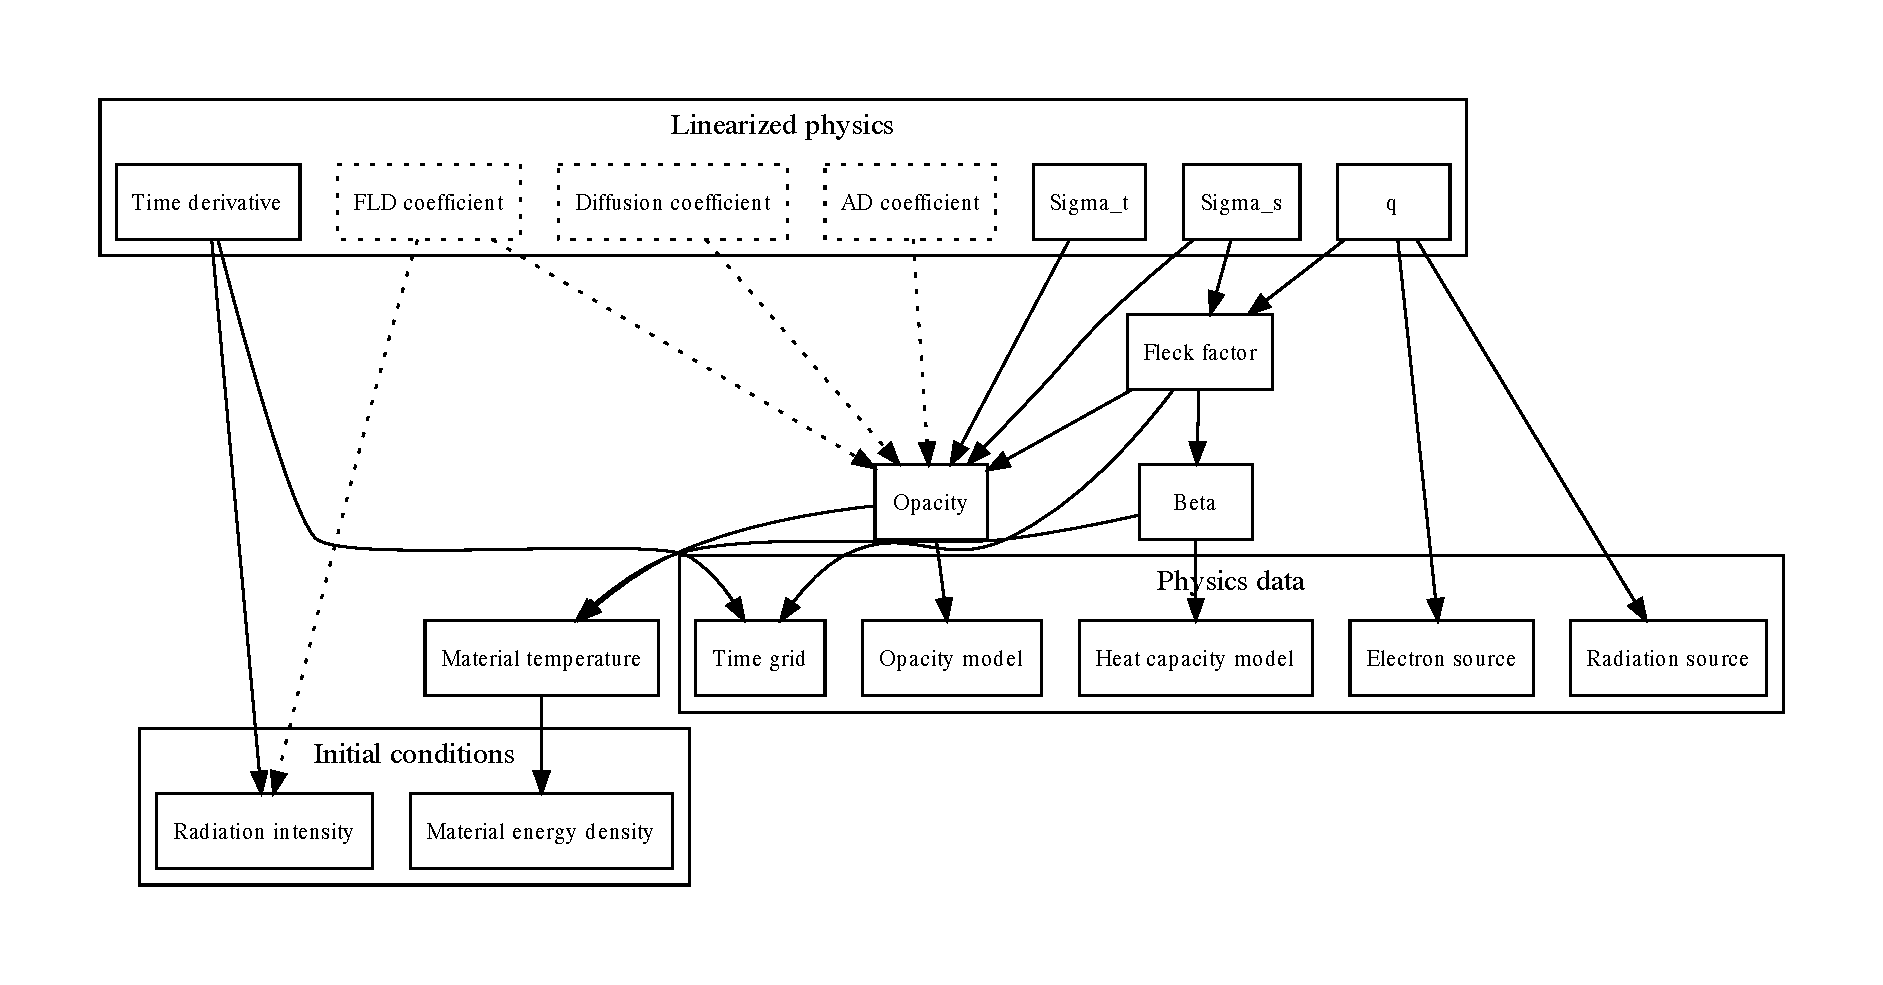
\includegraphics[width=8in]{semi-implicit}
  \caption{Dependency graph of quantities in the semi-implicit discretization.}
  \label{fig:semiImplicitFlowchart}
\end{sidewaysfigure}

